\section{Restoring the exchange geometry}\label{sec:control}

\subsection{Control laws}
By \cref{thm:absorption}, deep recurrent absorption requires bounded total
energy, $\eA$ near $0$, and $\psi$ locked near $\psis=(\tau+\sigma)\pi/2$.
\Cref{sec:mismatch} identified what threatens each of these:
\begin{itemize}
\item delay and sampling pump the fast mode, so $\eH$ grows (\cref{cor:delay-modal});
\item they drive $\eA$ at the constant rate $\alpha_\Sigma$, so $\eA$ drifts;
\item static common errors make $\psi$ drift (\cref{prop:static}).
\end{itemize}
\Cref{prop:authority} identified the common coupling as the effective actuator
for the phase.
All controller inputs are computed from the reconstructed state
$\hat x=(\hat q,\hat{\dot q},z,\dot z)$; hats denote reconstructed quantities.
The controller acts through the antisymmetric coupling $w$ and the common coupling
$c=s+c_\psi$ in \eqref{eq:realised}, with $\omega_z=1$:
\begin{subequations}\label{eq:control}
\begin{align}
  w&=-K_E\,\frac{\Hr}{\hat H^2}\,\hat e_H\,\hat g, \label{eq:u}\\
  s&=-\frac{K_A}{\hat H}\,(\hat e_A+\zeta_A)\,\hat m,
  &\dot\zeta_A&=k_{IA}\,\hat e_A, \label{eq:s}\\
  c_\psi&=-\frac{1}{\beta_\psi}\big(k_P\sin(\hat\psi-\psis)+\xi\big),
  &\dot\xi&=k_I\sin(\hat\psi-\psis), \label{eq:cpsi}
\end{align}
\end{subequations}
with gains $K_E,K_A,k_P,k_I>0$, $k_{IA}\ge0$, and $\beta_\psi$ from
\eqref{eq:psi-static}.
Here $\hat g=\hat{\dot q}\dot z$, $\hat m=\hat q\hat{\dot q}+z\dot z$, and $\hat
e_A$, $\hat\psi$ are obtained from $T\hat x$ by \cref{lem:modal}.
In the sampled implementation the right-hand sides are evaluated at $t_k$ and
held.

The laws have the following structure.
\begin{itemize}
\item \eqref{eq:u} injects the power $2w\dot q\dot z$ (by \eqref{eq:Hdot}),
  which opposes the energy error.
\item \eqref{eq:s} is power-neutral and redistributes energy between the modes
  through \eqref{eq:common-amp}; since $\hat m$ is zero-mean, $s$ has no
  first-order effect on the modal frequencies.
\item \eqref{eq:cpsi} is a proportional--integral phase-locked loop acting
  through the common-coupling sensitivity of \cref{prop:static}.
\end{itemize}
At $\hat H=\Hr$, \eqref{eq:u}--\eqref{eq:s} with $k_{IA}=0$ coincide with the energy
and amplitude laws of~\citet{juchem2027restoring}.
The normalisation by $\hat H$ makes them homogeneous of degree zero, matching
the linearity of the plant, and it turns the averaged gains in
\cref{lem:averaged} into functions of $\eA$ only.
The new elements are the integral action in \eqref{eq:s}, which is needed because
the delay-induced drift $\alpha_\Sigma$ is constant, and the phase loop
\eqref{eq:cpsi}, which replaces the virtual-stiffness adaptation.

\subsection{Ideal loops: exact convergence}
Without implementation errors, the isolated energy and amplitude loops converge
without any averaging or excitation assumption.

\begin{proposition}[Ideal loops]\label{prop:ideal}
Consider \eqref{eq:realised} with ideal channels, $\eta=f=0$, $\omega_z=1$ and
$\hat x=x$.
\begin{enumerate}
\item[(a)] With $s=c_\psi=0$ and \eqref{eq:u}: $\dot\eH=-2K_E(g/H)^2\eH$, and
  $\eH(t)\to0$ for every $x(0)\neq0$.
\item[(b)] With $w=c_\psi=0$, $k_{IA}=0$ and \eqref{eq:s}: $H$ is constant,
  $\dot\eA=-\tfrac{2K_A}{S}\sin^2\!\varphi\;\eA$ with $\varphi=\theta_++\theta_-$,
  and $\eA(t)\to0$ for every $x(0)\in\mathcal D_0$.
  Hence $A_\pm(t)\to\sqrt{2H(0)}/S$.
\end{enumerate}
\end{proposition}
\begin{proof}
(a) By \eqref{eq:Hdot}, $\dot H=2wg=-2K_E\Hr\eH g^2/H^2$; divide by $\Hr$.
Then $|\eH|$ is non-increasing, so $H(t)$ stays in a compact interval of
$(0,\infty)$ and $x(t)$ in a compact subset of $\RR^4\setminus\{0\}$, where the
autonomous closed loop is smooth.
By LaSalle's invariance principle, $x(t)$ converges to the largest invariant set
in $\{g\,\eH=0\}$.
On a solution in that set with $\eH\neq0$ we would have $g\equiv0$, hence $w\equiv0$,
so the solution is nominal.
By \cref{lem:modal}(5), $g\equiv0$ along a nominal solution forces
$A_+=A_-=0$, which contradicts $H>0$.
(b) $H$ is constant because $s$ is power-neutral.
By \eqref{eq:common-amp} and \cref{lem:modal}(4),
$\dot\eA=\dot A_+/A_+-\dot A_-/A_-=\frac{s\sin\varphi}{SA_+A_-}(\Om
A_-^2+\Op A_+^2)=\frac{2Hs\sin\varphi}{S^2A_+A_-}$, and substituting
\eqref{eq:s} gives the stated equation.
Since $|\eA|$ is non-increasing and $H$ is fixed, $A_\pm$ remain in a compact
subset of $(0,\infty)$.
On the invariant subset of $\{\eA\sin\varphi=0\}$ with $\eA\ne0$ we would have
$s\equiv0$, hence the nominal flow, along which $\dot\varphi=S\neq0$: a
contradiction.
Thus $\eA\to0$, and \cref{lem:modal}(3) gives the limit.
\end{proof}

Part (b) is the corrected form of~\citet[Prop.~2]{juchem2027restoring}
(see \cref{rem:ecc-fix}).
Part (a) shows that the energy loop needs no persistence-of-excitation
assumption: excitation is \emph{structural}, because $g\equiv0$ is incompatible
with non-zero energy on the nominal flow.
The quantitative counterpart is the next lemma.

\begin{lemma}[Structural excitation]\label{lem:pe}
If $\tau+\sigma\ge5$, then along every nominal orbit
\begin{multline}\label{eq:mubar}
  \frac{1}{P_0}\int_t^{t+P_0}g^2\,\dd\vartheta=\bar\mu(A_+,A_-)\\
  :=\frac{\Op^4A_+^4}{8}+\frac{\Om^4A_-^4}{8}+\frac{A_+^2A_-^2}{2},
\end{multline}
and $\nu(a):=\bar\mu/H^2=\tfrac{1}{2S^2}\big(\Op^2a^2+\Om^2(1-a)^2+4a(1-a)\big)$
satisfies $\nu_{\min}:=\Om^2/(2S^2)\le\nu(a)\le\nu_{\max}$ for all $a\in[0,1]$,
whenever $n<\sqrt2$.
\end{lemma}
\begin{proof}
Square the expression in \cref{lem:modal}(5).
The cross terms are harmonics $e^{\ii(k\theta_++l\theta_-)}$ with
$(k,l)\neq0$ and $|k|+|l|\le4$.
On the resonant orbit $k\Op+l\Om=0$ requires $(k,l)\in\ZZ(\sigma,-\tau)$, which
is impossible for $|k|+|l|\le4<\tau+\sigma$.
Their averages over $P_0$ therefore vanish.
Using \cref{lem:modal}(3) and \eqref{eq:share}, $\nu$ is a quadratic in $a$ with
leading coefficient $(S^2-6)/(2S^2)<0$ for $n<\sqrt2$.
It is concave, so its minimum is at an endpoint, $\min\{\Op^2,\Om^2\}/(2S^2)$.
\end{proof}

For $(11,9)$, $\nu\in[0.101,0.189]$, and \eqref{eq:mubar} reproduces the
excitation constant $\mu_{P_0}=2.95$ of~\citet{juchem2027restoring}.
The windowed excitation \emph{assumption} of the conference version is thus a
consequence of the geometry.

\subsection{First-order averaged dynamics}
In the slow-adaptation regime the closed loop has two time scales: the modal
phases rotate at $\Opm$, while $(H,\eA,\psi)$ and the integrators drift slowly.
Introduce a small parameter $\epsilon>0$ and scale
\begin{equation}\label{eq:scaling}
\begin{gathered}
  (K_E,K_A,k_P)=\epsilon(\bar K_E,\bar K_A,\bar k_P),\\
  (k_{IA},k_I)=\epsilon^2(\bar k_{IA},\bar k_I),\qquad d=\epsilon\bar d,
\end{gathered}
\end{equation}
with static errors $\eta_c,\eta_w=O(\epsilon)$.
In the rotating frame $\tilde\zeta_\pm=e^{-\ii\Opm t}\zeta_\pm$ the closed loop is
then in the standard form $\dot y=\epsilon F(t,y,v)$, with $F$ $P_0$-periodic in
$t$.
Here $v$ collects the measurement errors and mismatch.

\begin{assumption}[Measurement errors]\label{ass:meas}
The reconstruction errors are captured, to first order, by bounded biases
$\delta_H:=\avg{\hat e_H-\eH}$, $\delta_A:=\avg{\hat e_A-\eA}$ and
$\delta_\psi:=\avg{\hat\psi-\psi}$.
Zero-mean noise only enters at second order.
\end{assumption}

\begin{lemma}[Averaged closed loop]\label{lem:averaged}
Let $\tau+\sigma\ge5$ and $\omega_z=1$.
To first order in $\epsilon$, the average of the closed loop
\eqref{eq:realised}, \eqref{eq:control} in the coordinates
$(\eH,\eA,\zeta_A,\psi,\xi)$ is
\begin{subequations}\label{eq:avg}
\begin{align}
  \dot\eH&=-2K_E\,\nu(a)\,(\eH+\delta_H)+\omega_H(a)(1+\eH),\label{eq:avg-H}\\
  \dot\eA&=-\tfrac{K_A}{S}(\eA+\zeta_A+\delta_A)+\alpha_\Sigma\nonumber\\
    &\quad-\tfrac{2K_E}{S^2}\chi(a)\tfrac{\eH+\delta_H}{1+\eH},\label{eq:avg-A}\\
  \dot\zeta_A&=k_{IA}(\eA+\delta_A),\label{eq:avg-zeta}\\
  \dot\psi&=-k_P\sin(\psi-\psis+\delta_\psi)-\xi+\beta_\psi\eta_c,\label{eq:avg-psi}\\
  \dot\xi&=k_I\sin(\psi-\psis+\delta_\psi),\label{eq:avg-xi}
\end{align}
\end{subequations}
where $a=a(\eA)$ is the share \eqref{eq:share}, $\nu$ is as in \cref{lem:pe},
$\alpha_\Sigma=\alpha_\Sigma(d)$ is given by \eqref{eq:alpha-sigma}, and
\begin{align}
  \chi(a)&=\tfrac14\big(a(\Op^2-2)-(1-a)(\Om^2-2)\big),\label{eq:chi-omega}\\
  \omega_H(a)&=\tfrac{nd}{S}\big(\Op^2a-\Om^2(1-a)\big).\nonumber
\end{align}
\end{lemma}

The proof (\cref{app:averaged}) evaluates the torus averages of
\eqref{eq:Hdot}--\eqref{eq:thdot} term by term; the non-resonance condition
$\tau+\sigma\ge5$ removes every resonant harmonic.
The averaged model has three structural properties:
\begin{enumerate}
\item it is \emph{triangular}: $\eH$ does not depend on $(\zeta_A,\psi,\xi)$, and
  the phase loop is decoupled from the energy and amplitude loops;
\item the only cross-coupling, from $\eH$ into $\eA$, vanishes when
  $\eH+\delta_H=0$;
\item all coefficients depend on $\eA$ only through the bounded share
  $a\in(0,1)$.
\end{enumerate}
Second-order effects such as $\avg{s^2}$ and $\avg{w^2}$, which shift the modal
frequencies~\citep[eq.~(72)]{juchem2027restoring}, enter \eqref{eq:avg-psi}
as slowly varying disturbances; the integrator $\xi$ rejects them.
\Cref{fig:averaged} compares \eqref{eq:avg} with the exact sampled-data
simulation.
The predicted steady state $\eA^\star=S\alpha_\Sigma/K_A$ without integral action,
its removal with $k_{IA}>0$, and the transient of the phase loop with its trim
$c_\psi\to-\eta_c$ match to within a few percent.
\gap{Second-order accuracy of $\eH$}{The averaged steady state of $\eH$
underestimates the simulated mean by about 25\,\% for $(K_E,K_A)=(1,0.3)$ and by
a factor 3 for $(10,1)$ (code/scripts/fig\_averaged.py). Correlations between the
fast ripple of $\eH$ and $\hat g$ are second-order effects. Either derive the
second-order average or bound the discrepancy.}

\begin{figure*}[t]
  \centering
  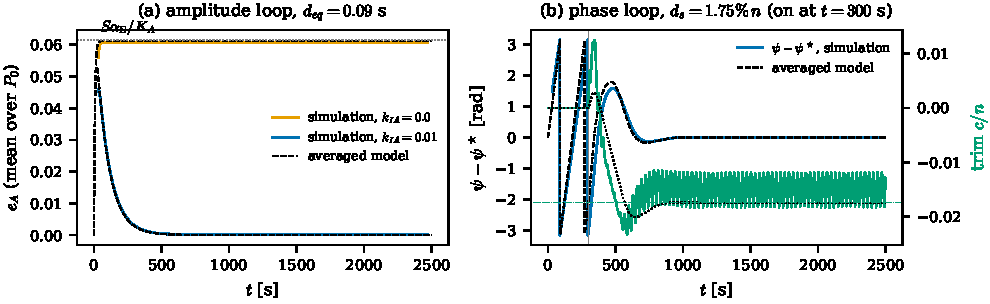
\includegraphics[width=\textwidth]{fig_averaged.pdf}
  \caption{Averaged model \eqref{eq:avg} (dashed) versus exact sampled-data
  simulation ($T_s=0.03$\,s, $k_y=k_a=1$, so $\deq=0.09$\,s; $K_E=1$, $K_A=0.3$).
  (a) $\eA$ averaged over $P_0$: without integral action it settles at
  $S\alpha_\Sigma/K_A$; with $k_{IA}=0.01$ it converges to zero.
  (b) Sensor and actuator gain errors $-3\,\%$ and $+6.5\,\%$
  ($\eta_c=1.75\,\%\,n$): $\psi$ drifts until the phase loop
  ($k_P=0.02$, $k_I=2\times10^{-4}$) is switched on at $t=300$\,s; the trim
  converges to $-\eta_c$.}
  \label{fig:averaged}
\end{figure*}

\subsection{Input-to-state stability of the averaged loop}
Let $h_0\in(0,\tfrac12)$ and $\mathcal E_{h_0}:=\{\eH\ge-1+h_0\}$.
We write $\bar\omega_H:=nd\Op^2/S\ge\sup_a|\omega_H(a)|$,
$\bar\chi:=\sup_a|\chi(a)|$, and $\tilde\zeta_A:=\zeta_A-S\alpha_\Sigma/K_A$.

\begin{theorem}[ISS of the averaged closed loop]\label{thm:iss-avg}
Consider \eqref{eq:avg} with $k_{IA}>0$ and suppose
\begin{equation}\label{eq:gain-cond}
  \lambda_H:=2K_E\nu_{\min}-\bar\omega_H>0,
  \quad\text{i.e.}\quad K_E>nd\,S\,\Op^4 .
\end{equation}
\begin{enumerate}
\item[(a)] \emph{Energy.} For $\|\delta_H\|_\infty\le1-2h_0$ the set
  $\mathcal E_{h_0}$ is forward invariant, and
  \begin{equation}\label{eq:iss-H}
    |\eH(t)|\le e^{-\lambda_Ht}|\eH(0)|
      +\frac{2K_E\nu_{\max}\|\delta_H\|_\infty+\bar\omega_H}{\lambda_H}.
  \end{equation}
\item[(b)] \emph{Amplitude.} On $\mathcal E_{h_0}$, the subsystem
  $(\eA,\tilde\zeta_A)$ is ISS with respect to $(\eH+\delta_H,\delta_A,\dot
  d)$, with linear gains.
  The cascade $(\eH,\eA,\tilde\zeta_A)$ is ISS with respect to
  $(\delta_H,\delta_A,d,\dot d)$.
  For constant inputs and sufficiently small $d$, the equilibrium satisfies
  $\eA=-\delta_A$ and is exponentially stable: integral action rejects the
  delay-induced drift.
\item[(c)] \emph{Phase.} For constant $\eta_c$ and $\delta_\psi$, every
  solution of \eqref{eq:avg-psi}--\eqref{eq:avg-xi} converges to an equilibrium.
  The equilibrium $(\psi,\xi)=(\psis-\delta_\psi,\beta_\psi\eta_c)$ is locally
  exponentially stable and attracts all initial conditions outside the
  one-dimensional stable manifold of the saddle
  $(\psis-\delta_\psi+\pi,\beta_\psi\eta_c)$.
  The trim converges to $c_\psi\to-\eta_c$.
\end{enumerate}
\end{theorem}

The proof (\cref{app:iss}) uses three ingredients.
Part (a) is a scalar comparison argument, since by \cref{lem:pe} the
coefficient of $\eH$ is at least $\lambda_H$.
Part (b) treats $(\eA,\tilde\zeta_A)$ as a Hurwitz linear system driven by a
bounded nonlinearity of the inputs, and uses the ISS cascade
theorem~\citep{sontag1989smooth}.
Part (c) uses the Lyapunov function
$V=k_I(1-\cos(\psi-\psis+\delta_\psi))+\tfrac12(\xi-\beta_\psi\eta_c)^2$,
whose derivative is $-k_Pk_I\sin^2(\cdot)\le0$, together with LaSalle and a
linearisation at the two equilibria.

Condition \eqref{eq:gain-cond} is mild: the energy gain must beat the
delay-induced anti-damping.
For $(11,9)$ and $\deq=0.09$\,s it requires $K_E>0.054$.
Part (a) also exposes a hard limit: a bias $\delta_H$ in the energy
reconstruction (e.g.\ a sensor gain error) is passed to $\eH$ with gain
$\nu_{\max}/\nu_{\min}$ and cannot be removed by feedback.
\gap{Almost-global ISS of the phase loop}{Part (c) is an asymptotic statement for
constant inputs. Upgrade it to almost-global ISS on $\mathbb S^1\times\RR$ with
respect to $(\dot\eta_c,\delta_\psi)$ in the sense of~\citet{angeli2004almost},
and give explicit local ISS gains. These are needed to bound the residual phase
error that enters \cref{rem:apex}.}

\subsection{From the averaged to the actual sampled loop}
ISS of the averaged system transfers to the original time-varying system in a
semiglobal practical sense~\citep{nesic2001input,teel2003unified}.

\begin{theorem}[Semiglobal practical ISS]\label{thm:spiss}
Let the assumptions of \cref{thm:iss-avg} hold for the scaled gains
\eqref{eq:scaling} and let $\mathcal K$ be a compact subset of
$\{x\in\mathcal D_0:\ \eH\ge-1+h_0\}$ such that $\psi(0)$ lies in a compact
subset of the basin of attraction in \cref{thm:iss-avg}(c).
Let $\chi:=(\eH,\eA,\tilde\zeta_A,\psi-\psis,\xi-\beta_\psi\eta_c)$.
Then for every input bound $\bar v$ and every $\nu>0$ there exists
$\epsilon^\star>0$ such that, for all $\epsilon\in(0,\epsilon^\star)$, all
initial conditions in $\mathcal K$ and all inputs with $\|v\|_\infty\le\bar v$,
the solutions of the actual closed loop satisfy
\begin{equation}\label{eq:spiss}
  |\chi(t)|\le\beta\big(|\chi(0)|,\epsilon t\big)+\gamma(\|v\|_\infty)+\nu
  \qquad\forall t\ge0,
\end{equation}
with $\beta\in\mathcal{KL}$ and $\gamma\in\mathcal K$ inherited from
\cref{thm:iss-avg}.
\end{theorem}

\begin{proof}[Proof (sketch)]
In the rotating frame of \cref{lem:averaged} the closed loop without delay is an
ODE $\dot y=\epsilon F(t,y,v)$ with $F$ $P_0$-periodic in $t$, locally Lipschitz
on $\mathcal K$, and with average equal to \eqref{eq:avg}.
\Cref{thm:iss-avg} gives ISS of the average on the relevant compact sets.
The result of~\citet[Thm.~2]{nesic2001input} then yields \eqref{eq:spiss}.
\end{proof}

\gap{Delay and sampling inside the averaging theorem}{The sketch covers the ODE
part. The loop delay and ZOH enter \cref{lem:averaged} through their
first-order expansion (\cref{cor:delay-modal}, \cref{prop:zoh}). Two rigorous
routes: (i) averaging for retarded functional differential
equations~\citep{lehman1999fundamental} with $d=\epsilon\bar d$; (ii) the exact
lifted discrete-time model of \cref{ass:sampled} with discrete-time averaging
and the sampled-data ISS framework of~\citet{nesic2004framework}. Route (ii)
seems cleaner because the plant model is then exact.}
\gap{Non-small gains}{The simulations in \cref{sec:sim} use the gains
of~\citet{juchem2027restoring} ($K_E=10$), which lie outside any explicit
$\epsilon^\star$. \Cref{prop:ideal}(a) shows that the energy loop converges for
every $K_E>0$ in the ideal case. A non-averaged ISS proof of the energy loop for
large $K_E$ should be possible: the scalar LTV equation for $\eH$ together with
\cref{lem:pe} and a bound on how fast $u$ changes the shape $(a,\varphi)$ of the
state.}
